\chapter{Implementation deatils}
\label{sec:impl}
Reviewernet is a fully client-side application. It builds on a bibliographic dataset extracted from a reference corpus containing more than 180 million records.

In this chapter, we describe our implementation choices: the data and the preprocessing  (Section \ref{sec:data}), languages, frameworks and external libraries used to deploy the user interface (Section \ref{sec:lang}); we conclude with an analysis of the code that implements additional features of our interactive visualization system (Section \ref{sec:misccode}).
\section{The data}
\label{sec:data}
To construct the reference dataset, we collected papers, authors and citations from eight selected sources in the field of Computer Graphics, taken from the Semantic Scholar Research Corpus \cite{ammar:18}. 

The original corpus currently contains more than 180 millions research papers published in all fields, provided as JSON objects, one per line. Archives are partitioned in batches and shared as a collection of gzipped files. In Figure \ref{jsonfields} there is the full list of the attributes of a generic record that represents a publication.

\begin{figure}[!ht]
    \centering
    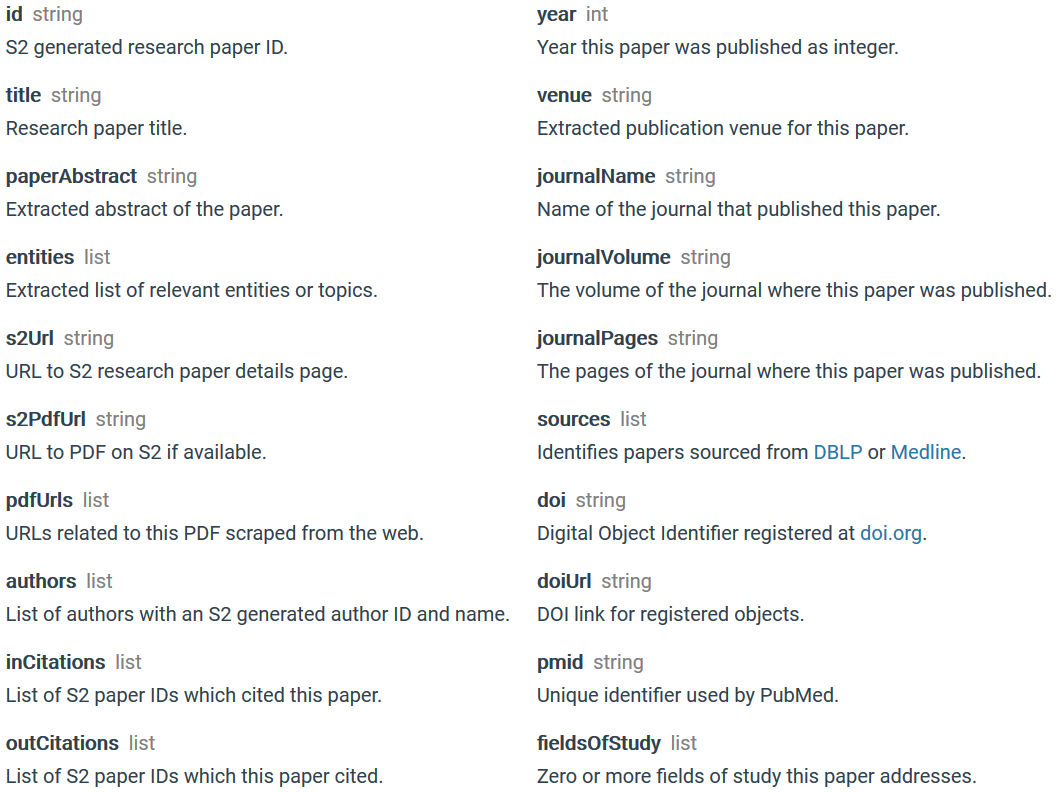
\includegraphics[width=\textwidth]{fig/corpusfields.png}
    \caption{Definition of attributes of the Semantic Scholar research corpus, from http://api.semanticscholar.org/corpus/. \label{jsonfields}}
\end{figure}

To demonstrate the application in the field of Computer Graphics, We filtered the corpus extracting only publications from journals and conference proceedings listed in Table \ref{table:sources}, spanning the years in-between 1995 and 2019. 

The final reference dataset contains 22.887 papers, 145.900 citations, and 29.549 authors.
\begin{table}[!ht]
\renewcommand{\arraystretch}{1.3}
\centering
\begin{tabular}{|l|c|}
\hline
ACM Transactions on Graphics & 2594\\ 
Computer Graphics and Applications  & 1697 \\ 
Computer Graphics Forum & 3521\\ 
Computers \& Graphics & 2092\\ 
IEEE Transactions on Visualization and Computer Graphics & 3638\\ 
Visual Computer & 2107\\ 
Proceedings of IEEE Conference Visualization (pre 2006) & 474 \\ 
Proceedings of ACM SIGGRAPH (pre 2003) & 6718\\
\hline
\end{tabular}
\caption{The selected sources from the Semantic Scholar Research Corpus used in our demonstration scenario. The final reference dataset contains 22.887 papers, 145.900 citations, and 29.549 authors.}
\label{table:sources}
\end{table}

%\input{stats.tex}
\subsection*{Pre-processing}
\label{sec:preproc}

The total size of the corpus is about 180 GB and the data quality is fairly good, but there's ambiguity in how journals and venues are referenced (acronyms, multiple abbreviations, ecc...) and there might be consistency problems in citations as extracted from JSON files. Hence the pre-processing phase is crucial to lower data complexity while maintaining coherence and topic coverage to properly support the reviewer selection process. 

After non-paper (such as acknowledgements to reviewers, prefaces, etc.) and useless attributes deletion, each single JSON has been parsed and filtered separately with a python script. In this filtering step, we use a string-matching algorithm to correctly assign papers to venues and journals (see Sections \ref{sec:lang} and \ref{sec:misccode}). Then we have the final consolidation step in which we:
\begin{itemize}
    \item check citations consistency, to ensure we only extract citations published in one of the venues in our reference list (Table \ref{table:sources});
    \item precompute co-authorship relathionships among researchers;
    \item merge the filtered data obtaining 3 JSON files (authors, papers, journals) representing the Computer Graphic reference corpus.
\end{itemize}

The \emph{papers' file} is a JSON representation of the PN. It contains two lists: \textit{nodes} and \textit{links}, representing respectively papers and citation relathionships. 
\begin{table}[!ht]
    \centering
    \begin{tabular}{ll}
    id {\color[HTML]{656565}string}    & paper ID.           \\ 
    value {\color[HTML]{656565}string} & Paper title.                      \\
    year {\color[HTML]{656565}int}     & Publication year of this paper.   \\
    authsId {\color[HTML]{656565}list} & List of S2 generated author IDs.  \\                
    jn {\color[HTML]{656565}string}                                          & Name of the journal that published this paper. \\
    j\_id {\color[HTML]{656565}string}                                        & ID of the journal.                             \\
    venue {\color[HTML]{656565}string}                                       & Extracted publication venue.                   \\
    v\_id {\color[HTML]{656565}string}                                        & Venue ID.                                      \\
    color {\color[HTML]{656565}int}    & Number of in-citations.            \\  
    nOc {\color[HTML]{656565}int} & Number of out-citations. 
\end{tabular}
    \caption{Definition of attributes of the generic node in the PN. \label{tab:nodes}}
   
    \end{table}

    The node entity is essentially the same as in the reference corpus with less attributes, as described in Table \ref{tab:nodes}. The link object is simpler: for each citation in the dataset we have the source and target ID. 
    
    The \emph{authors' file} is a list of JSON, one for each researcher. Table \ref{tab:authors} describes the author entity in ReviewerNet.

\begin{table}[!ht]
    \centering
    \begin{tabular}{ll}
    id {\color[HTML]{656565}string}    & researcher ID.           \\ \hline
    value {\color[HTML]{656565}string} & Researcher name.                      \\ \hline
    lastPub {\color[HTML]{656565}list}     & \begin{tabular}[c]{@{}l@{}}List containing the researcher last publication's year\\and ID, in the extracted dataset.\end{tabular}\\ \hline
    paperList {\color[HTML]{656565}list} & \begin{tabular}[c]{@{}l@{}}List of papers' IDs authored by this researcher\\in the extracted dataset.\end{tabular}\\    \hline         
    coAuthList {\color[HTML]{656565}dict} & \begin{tabular}[c]{@{}l@{}}A dictionary with one entry for each co-author\\of the researcher. Each dictionary element contains\\pre-computed information about the shared works\\between the two researchers in the dataset. \end{tabular}
\end{tabular}
    \caption{List and description of researchers' attributes in the ReviewerNet representaion. \label{tab:authors}}
   
    \end{table}

The \texttt{coAuthList} field is a fondamental one: it allows one to rapidly discover conflicts among researchers, easing the real-time computation load.

The \emph{journals' file}, eventually, contains information about the venue names consolidation and useful statistics. For each entity we store:
    \begin{itemize}
        \item venue unique ID;
        \item a list of names and achronims that refers to the journal/venue; this list is used in the approximate string matching routine;
        \item the number of papers, authors and citations, collected with the reference list \ref{table:sources};
        \item a pre-computed \emph{venue score}, that is the total number of in-citations, over all the venue publications, coming from a different venue; this score is used to decide in which order the venues will be showed to the user and in the corresponding color-map.  
    \end{itemize}

This file is loaded first once the user chooses the instance upon which to run a ReviewerNet session and is used to quickly print statistics about the instance, without loading the entire dataset.
\section{Languages \& external libraries}
\label{sec:lang}

Our visualization system is fully client-side, meaning it is a web page and the bibliographic database is fully loaded and queried on the local client.

For downloading and pre-processing the data we run a bash script that downloads the gzipped partitions and executes python scripts in parallel to process them. The only external dependency in this phase is the string matching python library \emph{fuzzywuzzy}\footnote{\url{https://github.com/seatgeek/fuzzywuzzy}} that performs the approximate string matching of venues names. We chose this approach to overcome ambiguity problems in the data (see Section \ref{sec:data}).

The static part of the website is mainly written in HTML5 and CSS, while for the dynamic one we use Javascript. In the user interface, we also use Bootstrap v3.3.7 responsive and adaptive components and JQueryUi v1.12.1 search-bars and widgets.

Finally, the core external library is D3.js v4.13.0: a JavaScript library for visualizing data using web standards that combines powerful visualization and interaction techniques with a data-driven approach to DOM manipulation \cite{D3js11}. We use it for graph drawing (PN and RN) and for managing the data-driven visualization in general - e.g. the code lines that implement nearly all the available user interactions, described in Section \ref{subsec:actions}, are calls to this library.

Concerning graph drawing, the PN is a fixed-layout force simulation, while nodes in the RN are free to move and their position is computed with a many-body (or $n$-body) force simulation. It can be used to simulate gravity (attraction) if the strength is positive, or electrostatic charge (repulsion) if the strength is negative. In order to highlight research communities in the RN, we chose to charge the nodes with a repulsive force, while links attract them proportionally to the number of shared papers. This configuration of the force simulation enhances clustering of \virgolette{close} researchers and communities. 

The D3 implementation of the n-body simulation uses quadtrees and the Barnes-Hut Approximation \cite{Barnes1986} to improve performance.

\section{Additional features}\label{sec:misccode}
ReviewerNet is a visualization platform, but it integrates additional functionalities that the user can exploit to adapt the application to his/her needs and also to speed up the process in general.

\paragraph*{Export and load a ReviewerNet session}
As soon as the user starts to populate one of the networks or views, it is possible to download a plain-text file representing the current ReviewerNet session. The session file contains information about the parameter values (see Chapter \ref{sec:userinterface}), along with submitting, conflicting and candidate reviewer researchers selected and key papers. For each researcher/paper we store both id and name/title because IDs referring to the same entity may vary across different corpus snapshots; in this way, if, for example, the ID of a researcher in the sessions file is no longer valid, ReviewerNet shows an infromative pop-up that reports the name/title of missing researchers/papers, allowing the user to manually find it with the searchbars.     

The user can download the session file with a mouse click either on the \virgolette{Export Session} button in the CP or in the page footer. If the button in the CP is clicked, ReviewerNet will also report reviewers’ names and bibliographic references to their papers (see Chapter \ref{sec:demonstration} and Figure \ref{fig:list}).

Now, if a user reloads the page and still wants to work on one of his/her previous sessions, with a mouse click on the \virgolette{Import Session} button in the page footer it is possible to load any session file generated by the platform.

\paragraph*{Automated key papers insertion}
Manually initializing the PN with a set of seed documents can sometimes be time consuming, hence we introduced in ReviewerNet the possibility to automatically add papers to the visualization. 

The intuition is that the list of references in the submitted paper or in previously identified seed papers can provide a convenient strategy to initialize the network.

A mouse click on the \virgolette{Import from bibliography} button in the CP opens a textbox in which the user can copy and paste a set of reference directly from a PDF file. Then, with a mouse click on the \virgolette{Parse} button in the same window, the system returns the list of matching papers in the dataset, and the user can choose which one of the matching papers to include in the visualization (See Figure \ref{fig:keypapers_2}).

Given a reference pasted from a PDF, our parsing and matching routine initially performs string cleaning and then extracts the 3 best matching papers in the dataset, if any, with a score.

The score depends on the number occurrence of words in the paper's title. The main data structures that enable the scoring and matching are two dictionaries:
\begin{enumerate}
    \item the first stores, for each word in each papers title, the paper in which it occurred. This dictionary is precomputed when the data is loaded;  
    \item the second is a dictionary of counters, with one entry for each paper that matches one ore more word in the reference title; this dictionary instead is dynamically computed during the import procedure.
\end{enumerate}  

So when parsing a reference, for each word, we check if a dictionary entry exists, if so we increment the counters of the papers listed in the word's dictionary entry. When all the words in the reference have been processed, the 3 best matching papers are returned and the best matching one in shown.

\paragraph*{Generating a custom ReviewerNet instance}

For our demonstration, we extracted the publications in the reference dataset from 8 selected sources, all in the field of Computer Graphics. However, if the user feels there are missing venues or simply wants to instantiate the application over a completely different field, ReviewerNet can be built over \emph{any} subset of the Semantic Scholar corpus and customized to include the venues of interest.  

We developed a user-friendly procedure to build a customized instance of ReviewerNet that is basically the implementation of the pre-processing steps described in Section \ref{sec:preproc}. The code is available on \url{https://github.com/cnr-isti-vclab/ReviewerNet/tree/master/parser}.

Our solution consists of 5 files: 
\begin{enumerate}
\item \texttt{download\_and\_parse.sh}, the main file: a bash scripts that downloads each single JSON and runs in parallel python scripts to process the data;
\item \texttt{parse\_and\_filter.py}, a python script that filters a single JSON with the approximate string matching algorithm (see Section \ref{sec:lang});
\item \texttt{merge\_data.py} , a python script that consolidates and merges the data as filtered from the corpus;
\item \texttt{journals.txt}, a plain-text JSON file that contains the reference list of venues for which we want to extract the publications; for each venue we store an ID and a list of possible names with which the venue is referred in the corpus - we need this information to solve the ambiguity problem with the venue names (see Section \ref{sec:data});
\item \texttt{util.py}, a python library containing all functions and methods that implement parsing, filtering and merging routines.
\end{enumerate}

To get a personalized instance of Reviewernet, the user has to open \texttt{journals.txt} with a text editor and change the content of the JSON object with the names of the venues that will be used to build the topic-based datasets; then, he/she can run \texttt{download\_and\_parse.sh}.

The provided script downloads and parses the partitions in parallel, allowing a maximum number of 10 concurrent downloads and parsers. The output is:


    \begin{itemize}
        \item 180 corpus partitions as gzip files;

        \item at most 180 parsed files ending with \virgolette{\emph{-filtered}} suffix;
    \end{itemize}

When all partitions have been downloaded and filtered the merging phase can start: filtered corpus partitions are merged together and the personalized dataset is built. Eventually the script asks the user whether to delete or not the interemediate files (gzipped/filtered partitions).

At this point the \texttt{datasets} folder will contain the files needed to run ReviewerNet - that are the authors, papers and journals files (cf. Section \ref{sec:data} for details)- ending with \virgolette{\emph{\_pers}} suffix. To use the your customized dataset just start a local or remote ReviewerNet session and, in the starting page, click on the \virgolette{\emph{Upload instance}} button and select the three files just created.
